\documentclass[10pt,twoside,a4paper]{article}

% Configure these parameters.
% Name and email
\newcommand{\studentname}{Joe Yan}
\newcommand{\studentemail}{zy275@cam.ac.uk}

% Date work done
\newcommand{\svworkdate}{2017-5-11}

% Details of supervision
\newcommand{\svcourse}{CST Part IA: Numerical Method}
\newcommand{\svnumber}{1}
\newcommand{\svdate}{2016-5-13}
\newcommand{\svtime}{}
\newcommand{\svvenue}{Churchill 1C}
\newcommand{\svrname}{Dr John Fawcett}
\newcommand{\svrinit}{JKF}
% End configuration

\usepackage{a4}             % Adjust margins for A4 media
\usepackage{pgfplots}
\usepackage{fancyhdr}
\renewcommand{\headrulewidth}{0.4pt}
\renewcommand{\footrulewidth}{0.4pt}
\fancyheadoffset[LO,LE,RO,RE]{0pt}
\fancyfootoffset[LO,LE,RO,RE]{0pt}
\pagestyle{fancy}
\fancyhead{}
\fancyhead[LO,RE]{{\bfseries \studentname}\\\studentemail}
\fancyhead[RO,LE]{{\bfseries \svcourse, SV~\svnumber}\\\svdate\ \svtime, \svvenue}
\fancyfoot{}
\fancyfoot[LO,RE]{For: \svrname}
\fancyfoot[RO,LE]{\thepage\ / \pageref{LastPage}}
\fancyfoot[C]{}

\usepackage{lastpage}       % "n of m" page numbering
\usepackage{lscape}         % Makes landscape easier
%\usepackage{portland}      % Switch between portrait and landscape
\usepackage{graphics}       % Graphics commands
\usepackage{wrapfig}        % Wrapping text around figures
\usepackage{epsfig}         % Embed encapsulated postscript
\usepackage{rotating}       % Extra graphics rotation
%\usepackage{tables}        % Tabular environments
\usepackage{longtable}      % Page breaks within tables
\usepackage{supertabular}   % Page breaks within tables
\usepackage{multicol}       % Allows table cells to span cols
\usepackage{multirow}       % Allows table cells to span rows
\usepackage{texnames}       % Macros for common tex names
%\usepackage{trees}         % Tree-like layout
\usepackage{hhline}         % Horizontal lines in tables
\usepackage{siunitx}        % Correct spacing of units

\usepackage{listings}       % Source code listings
\usepackage{array}          % Array environment
\usepackage{hyperref}       % URL formatting
\usepackage{amsmath}        % American Mathematical Society
\usepackage{amssymb}        % Maths symbols
\usepackage{amsthm}         % Theorems
%\usepackage{mathpartir}    % Proofs and inference rules
\usepackage{verbatim}       % Verbatim blocks
\usepackage{ifthen}         % Conditional processing in tex
\usepackage{xcolor}         % X11 colour names

% control width and vertically align text in table cells
\newcolumntype{L}[1]{>{\raggedright\let\newline\\\arraybackslash\hspace{0pt}}m{#1}}
\newcolumntype{C}[1]{>{\centering\let\newline\\\arraybackslash\hspace{0pt}}m{#1}}
\newcolumntype{R}[1]{>{\raggedleft\let\newline\\\arraybackslash\hspace{0pt}}m{#1}}

% make hyperref links not-ugly
\hypersetup{
    colorlinks=false,
    pdfborder={0 0 0},
}

\renewcommand{\oddsidemargin}{-20pt}
\renewcommand{\evensidemargin}{-20pt}
\renewcommand{\topmargin}{-30pt}
\renewcommand{\textwidth}{410pt}
\renewcommand{\marginparwidth}{100pt}

\setlength{\parindent}{0em}
\addtolength{\parskip}{1ex}

\usepackage[draft]{changes}
\setauthormarkup[left]{\textbf{[#1]}~}
\definechangesauthor[\svrname]{\svrinit}{orange}
\newcommand{\jkfadd}[1]{\added[\svrinit]{#1}}
\newcommand{\jkfdel}[1]{\deleted[\svrinit]{#1}}
\newcommand{\jkfrep}[2]{\replaced[\svrinit]{#1}{#2}}
\newcommand{\jkfmar}[1]{\marginpar{\jkfadd{#1}}}

\lstset{basicstyle=\footnotesize\ttfamily,breaklines=true}
\lstset{framextopmargin=50pt}

\begin{document}

\author{\studentname}
\title{\svcourse, SV~\svnumber}
\date{\svworkdate}

\textbf{\svcourse, SV~\svnumber}\\
\textbf{\studentname}\\
\textbf{\svworkdate}\\

\section*{}
You are building a mobile phone app for KuDoS. 
\begin{itemize}
\item
Identify the subjects, people and principals involved in the system. 
\\A subject is a physical person involved in the project. E.g. A student or a supervisor under the meaning of a physical or natural person using the Kudos are all subjects to the Kudos.
\\A person is a natural or legal person. Other than a subject which just means a natural person, a person can also be the department, company or other entities which has legal rights and obligations. E.g. The Churchill College can be a person of Kudos because it has the obligation to provide supervision rooms.
\\A principle is a person, a (complex) role, an equipment, a communication channel or a compound of other principles. 
\\A role is an identity of someone or something in the project. E.g. A physical person can act as either a developer or a supervision to Kudos. It is possible that the same physical person has different roles. 
\\An complex role is the compound of multiple roles.
\\An equipment can be the server Kudos running on or a printer which prints supervision work.
\\A communication channel is the channel which the project uses to pass the information. E.g. the Internet the a communication channel for Kudos, the supervision booking information is passed on it.
\item
Where are there obligations of confidentiality? 
\\The obligation of confidentiality is the action of legally or morally protection to the secrets of someone else.
\\E.g. Students have the obligation not to spread the material provided by the supervisor without permission. Supervisors have the obligation not to break the past paper answer policy to provide the student the answer directly which they do not have the right to access.
\item
Give examples of what might constitute each of the following in an implemented system: error, failure, accident, hazard, risk, safety. 
\\An error is a design flaw or a deviation from the intended state. E.g. If the design ignore the consistency issue when two students send two colliding booking requests to the system at the same moment, it is possible that the system sends two booking conformation email but actually only one booking was successful.
\\A failure is a non-performance of the system. E.g. If the raven login authorisation server is down for some reason, it will cause a failure for student users which gives no respond for a login request. Student users now can not book or review their supervision information.
\\An accident is an undesired, unplanned event resulting in a loss. E.g. A malicious software successfully format the disk of the supervision booking information. If there are no backup, this will cause a permanent booking information loss, students can only rebook everything.
\\A hazard is a set of conditions on the system and the environment which can lead to a accident in the event of failure. E.g. The server which is running Kudos and supporting SSH use a weak password instead of set a key for remote login. There is a potential that someone may crack in the server and do something undesired.
\\Risk is the probability of an accident combined with its danger and duration. Shortly, it is the expectation of the damage may happen to the system.
\\Safety is the freedom from accidents.
\item
Provide a threat model and a fault-tree analysis. 
\\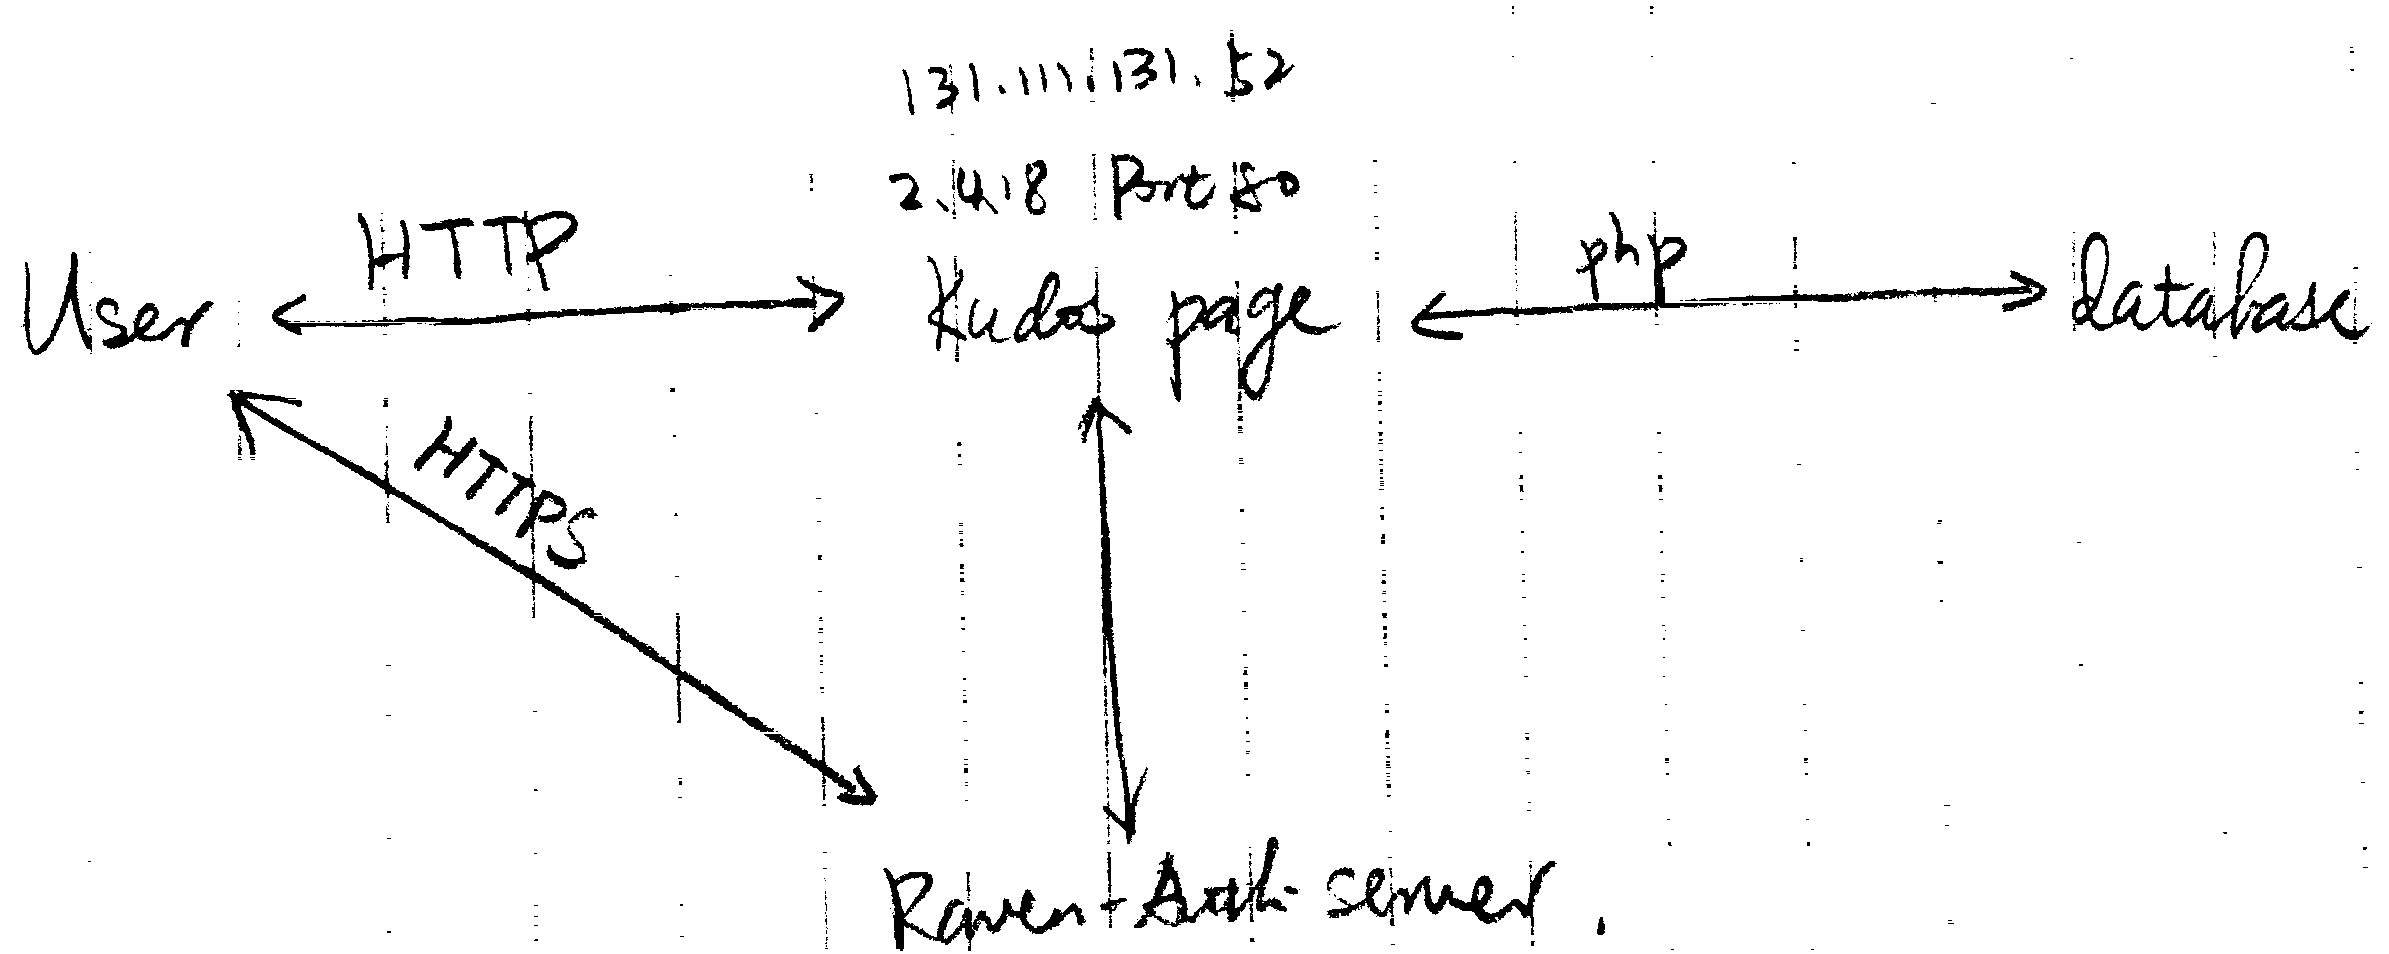
\includegraphics[scale=0.1]{IMG_1042.png} 
\\The connection between users and the Kudos page is not encrypted which may leak booking information.
\\The authorisation is based on the user device cookie which may allow a illegal login by cookie leak.
\\The $php?$ request is used which can be potentially abused. E.g. php?/etc/passwd
\begin{itemize}
\item Human failure
\begin{itemize}
\item weak password or leaked password
\item forget to logout on a public device
\item print a very long fake pdf from a April Fool joke (unlikely)
\end{itemize}
\item Protocol failure
\begin{itemize}
\item HTTP not encrypted
\item php? request abused
\item Other potential internet attack..
\end{itemize}
\item Device failure
\begin{itemize}
\item the server is physically damaged
\item printer out of ink
\end{itemize}
\item Outside support failure
\begin{itemize}
\item mid-man attack by weak college route protection
\item  raven authorisation server down
\end{itemize}
\end{itemize}
\item
Give an examples for each of decoupling policy from mechanism; and defence in depth.
\\Decoupling policy from mechanism means separation of requirement and the technical implementation.
\\E.g. A security mechanism will set up the access control and then the specific student user can book supervisions in which group. However, a policy tells which user should be able to book supervisions.
\\Defence in depth is based on cheese model which means failure can only happen when a series of failures at the same point in all defence layers happen at the same time. This greatly reduces the probability of failure comparing with only one layer of defence.
\\E.g. A student can login by raven account this is one layer of defence. It is possible to set up a mechanism if the account is logged in from a suspicious IP address then Kudos will require a conformation message from a email to a student's personal email address (not using the university email because it is also based on raven). This is a two layers defence to a illegal login.
\end{itemize}
\end{document}

